% !TeX program = xelatex
% Primary timings and scores: research/peer_crossover/evidence/paired-cases.csv.
% Fixed-width ablation: research/lowdim/peer_evidence/cases.csv.
\documentclass[11pt,a4paper]{article}
\usepackage[margin=25mm,top=21mm,bottom=21mm]{geometry}
\usepackage{fontspec}
\setmainfont{Latin Modern Roman}
\usepackage{amsmath,amssymb,booktabs,array,tabularx,microtype}
\usepackage{graphicx,placeins}
\usepackage[hidelinks]{hyperref}
\newcommand{\papertitle}{Feature selection with single-peer ridge gains}
\hypersetup{pdftitle={\papertitle},pdflang={en},pdfauthor={}}
\setlength{\emergencystretch}{1em}
\setlength{\tabcolsep}{5pt}
\renewcommand{\arraystretch}{1.12}
\renewcommand{\topfraction}{.88}
\renewcommand{\floatpagefraction}{.75}
\renewcommand{\textfraction}{.10}
\setlength{\textfloatsep}{12pt plus 2pt minus 2pt}
\setlength{\intextsep}{10pt plus 2pt minus 2pt}
\setlength{\abovecaptionskip}{5pt}
\setlength{\belowcaptionskip}{6pt}
\newcommand{\gain}{g}
\newcommand{\Full}{\textnormal{Full}}
\newcommand{\Ftest}{\textnormal{F}}
\newcommand{\tabnote}[1]{\par\smallskip\begin{minipage}{.96\linewidth}\footnotesize #1\end{minipage}}
\begin{document}
\begin{center}
\parbox{\linewidth}{\centering\LARGE\bfseries \papertitle\par}
\end{center}
\begin{abstract}
Each of two correlated features can predict a response well yet contribute little once the other is present. We rank each feature by the smaller of two reductions in penalized training loss. The first is the feature's gain when used alone in a ridge model. The second is its mean gain when added to each possible single peer. The concentration of these scores determines how many columns to retain. We evaluated the same rule on 387 classification and regression configurations with 4 to 54\,877 input columns. It removed columns in 384 configurations and finished selection, fitting and prediction sooner than full-feature ridge in 231. With the further requirement that the test score equal or exceed the full-feature score, 106 configurations qualified, compared with 102 for a width-matched F filter and 76 for a uniform random subset. Allowing a score loss of 0.02 gave counts of 155, 128 and 159, respectively. In a separate fixed-width comparison on 31 low-dimensional configurations, adding the peer gains improved two test scores and lowered one.
\end{abstract}
\noindent\textbf{Keywords}\quad feature selection, ridge regression, conditional marginal contribution, runtime

\section{Introduction}
Abalone and Diabetes both have ten columns in our experiments. An Abalone training split contains about 2,800 observations, compared with about 300 for Diabetes. Dropping a column therefore saves a different amount of work in the two regressions. On Diabetes, even a selector that identifies useful predictors has little time to pay for itself. Fitting and predicting with all ten columns takes about a millisecond. We measure elapsed time from receiving the feature matrices to producing test predictions. To assess which columns the selector finds, we also compare methods that retain exactly the same number.

Two correlated measurements can each predict a response well on their own. How much does one still contribute after fitting the other? Cohen et al.~\cite{cohen} measured feature contributions by the change in classification performance when a feature joins a coalition. We ask a narrower question for ridge models. We measure the decrease in penalized training loss when a candidate enters alone and when it joins a model containing one other feature. Taking the smaller of the gain in isolation and the mean gain with a peer discounts features whose contribution falls in the presence of other predictors.

We call this the \emph{single-peer rule}. Cross-products give the conditional gain for every pair of features without a separate ridge fit for each pair. The number of pairs grows quadratically with the input width. We therefore measure the cost of computing the ranking along with the savings from fitting the final model on fewer columns. We use the same ranking and width rule across all input sizes, compare it with a univariate F filter and random subsets at matched widths, and examine the contribution of peer gains at fixed width on a subset of the benchmark.

Two related approaches illustrate how the choice of utility affects feature selection. Zhao, Liu and Parilina~\cite{zhao} estimate feature contributions using a fitted model and a graph of feature relationships, then train the final predictor on the retained columns. Kaur et al.~\cite{kaur} evaluate candidate subsets under a strategic loss when individuals can respond to the deployed predictor. Our observations are fixed. We score candidate features by an in-sample reduction in penalized loss, then evaluate the selected columns by held-out predictive performance and elapsed time.

\section{Single-peer feature selection}\label{sec:method}
Let the training matrix have $n$ rows and $p$ columns. A \emph{peer} is a feature already included when evaluating the gain from adding candidate $j$. Write $S$ for the set of peers, with $j\notin S$. The single-peer rule uses a sample of $m=\min(n,768)$ training rows. If $n>m$, it divides the row indices, in their existing order, into $m$ consecutive intervals of approximately equal length and draws one row uniformly from each interval using a fixed seed. It uses every row otherwise. This sampling rule uses row order alone. Within the sampled rows, we center each feature and divide by its population standard deviation, mapping constant columns to zero. Denote the resulting matrix by $Z$. The response $Y$ is standardized in the same way for regression. For classification, its columns are centered one-hot class indicators.

\subsection{Gains with zero or one peer}
With penalty $\lambda=\sqrt m$, let $L(S)$ be the minimum ridge objective~\cite{ridge} on the sampled rows. The gain from adding feature $j$ is the drop in this objective after refitting the coefficients of all included columns,
\begin{equation}
 L(S)=\min_W\bigl\{\|Y-Z_SW\|_F^2+\lambda\|W\|_F^2\bigr\},
 \qquad \gain_j(S)=L(S)-L(S\cup\{j\}).\label{eq:loss}
\end{equation}
Set $A=Z^\top Z+\lambda I$ and $B=Z^\top Y$, and write $B_j$ for row $j$ of $B$. The gains with an empty peer set and with a single peer $k$ are
\begin{align}
 \gain_j(\varnothing)&=\frac{\|B_j\|_2^2}{A_{jj}},\label{eq:empty}\\
 \gain_j(\{k\})&=
 \frac{\|B_j-(A_{jk}/A_{kk})B_k\|_2^2}
 {A_{jj}-A_{jk}^2/A_{kk}},\qquad k\ne j.\label{eq:peer}
\end{align}
Equation~\eqref{eq:empty} is the scalar ridge solution. Equation~\eqref{eq:peer} uses the standard Schur complement. Eliminating the coefficient of $k$ leaves curvature $A_{jj}-A_{jk}^2/A_{kk}>0$ for $j$, and completing the square gives its gain. Pahikkala et al.~\cite[Eq.~(8)]{pahikkala} used a related rank-one inverse update to score candidate features by leave-one-out error in greedy ridge selection, implemented in RLScore~\cite{rlscore}. Here each conditional gain measures the decrease in the penalized training objective for a particular peer.

With $c$ response columns, forming the dense feature cross-products takes $O(mp^2)$ operations, and evaluating the gains from them takes $O(cp^2)$. Forming $B$ by dense matrix multiplication adds $O(mpc)$. For $p\le32$ the compiled kernel accumulates one triangle of the Gram matrix in a single pass. At $m=768$ and $p=32$, the leading $mp^2$ term is bounded by $768\cdot1{,}024$ and the triangular calculation requires $768\times528=405{,}504$ product accumulations. There are $32\times31=992$ ordered candidate--peer pairs.

\subsection{Ranking features and choosing the width}
For $p\ge2$, the score for candidate $j$ is the smaller of its empty-set gain and its mean gain across the $p-1$ possible single peers,
\begin{equation}
 s_j=\min\left\{\gain_j(\varnothing),\;
           \frac{1}{p-1}\sum_{k\ne j}\gain_j(\{k\})\right\}.
 \label{eq:score}
\end{equation}
For $p=1$, only the empty-set gain is used. If at least one score is positive, the selector retains
\begin{equation}
 K=\left\lceil\frac{(\sum_j s_j)^2}{\sum_j s_j^2}\right\rceil
 \label{eq:width}
\end{equation}
features. This width reflects the concentration of the scores. For example, if exactly $r$ features have equal positive scores and all remaining scores are zero, then $K=r$. We take the $K$ highest-scoring columns, breaking ties by the smaller original column index. All-zero scores return all features and count as a failure to reduce width. Both the ranking and the width are determined from training data alone.

For a nonconstant regression target and nonconstant feature, let $r_j$ be their correlation on the sampled rows. Standardization gives $\gain_j(\varnothing)=m^2r_j^2/(m+\sqrt m)$. For $m>2$ and finite F statistics, ranking by this gain gives the same ordering as univariate regression F on those rows. The conditional gains can discount the marginal gain, but averaging limits the effect of any one peer. Suppose $p>1$ and feature $j$ has a nonzero sample inner product with at most $d_j$ other columns. Then
\begin{equation}
 \left(1-\frac{d_j}{p-1}\right)\gain_j(\varnothing)
 \ \le\ s_j\ \le\ \gain_j(\varnothing).\label{eq:bound}
\end{equation}
Each orthogonal peer contributes exactly $\gain_j(\varnothing)$ in~\eqref{eq:peer}. The other gains are nonnegative, which gives the lower bound after averaging. The upper bound follows from~\eqref{eq:score}. In particular, if $B_j=0$, candidate $j$ scores zero even when a specific peer gives it a positive conditional gain. The bound concerns exact sample orthogonality. We examine changes in the selected columns empirically in Section~\ref{sec:res}.

\subsection{Computing the same scores on wide matrices}
Above 32 columns the implementation processes the cross-products in tiles of at most 512 columns per side. Each off-diagonal entry supplies the gains in both directions, adding $j$ to $k$ and adding $k$ to $j$. The implementation accumulates the two contributions and releases the tile. This bounds the size of the temporary Gram matrix while evaluating the full mean in Eq.~\eqref{eq:score}.

For sparse sampled inputs, a constant peer leaves a candidate's gain unchanged. Identical sparse columns can share a calculation, as can columns whose only nonzero entries occur in the same sampled row. After standardization the latter agree up to sign. Each group contributes with its original multiplicity, excluding the candidate itself. The mean still has $p-1$ terms. As a numerical check, we also compiled the small-matrix kernel with its array bound raised to 128. Across eight dense or sparse checks at widths 33, 64 and 101, including a spectroscopy split, both implementations selected the same column indices.

\section{Experimental design}\label{sec:exp}
\subsection{Data, splits and predictors}
We evaluated the single-peer rule and its comparators on 52 named data sources or prediction tasks and 25 simulation settings. A configuration specifies a task, a train--test split, a seed and a modeling protocol. The 387 configurations comprised 178 binary classification, 62 multiclass classification and 147 regression comparisons. Training sets ranged from 100 to 182\,276 rows and input matrices from 4 to 54\,877 columns. Table~\ref{tab:cohorts} gives the splits and replications for each benchmark group. Some named tasks share a source. For example, the near-infrared spectroscopy tasks include measurements of the same type of sample in different harvest seasons. Madelon is an artificial feature-selection challenge. Matching the training matrix, training labels, test matrix and test labels by their four fingerprints yielded 301 distinct sets of inputs.

\begin{table}[htbp]\centering\small
\caption{Benchmark composition. Each configuration fixes the task, data split, seed and modeling protocol. Several configurations can share a test set.}\label{tab:cohorts}
\begin{tabularx}{\linewidth}{@{}l r >{\raggedright\arraybackslash}X@{}}
\toprule
Benchmark group & Count & Sampling or replication scheme \\
\midrule
Tabular and sensor data & 69 & Archived train--test splits from 13 sources, including Abalone, Diabetes, HAR and SECOM.\\
Additional data and simulations & 57 & Three configurations each for five named sources and 14 simulation settings.\\
Repeated holdouts & 40 & Five seeded 75/25 splits for each of four binary, two multiclass and two regression tasks.\\
Ten-source tabular study & 30 & Three splits per source, using the ordinary ridge model from the four-stage study.\\
Dense features and speech & 19 & Handwritten digits, acoustic features and sensor data, using the original held-out observations or speakers.\\
Near-infrared spectroscopy & 36 & Twelve regression tasks, each with a fixed train--test split and three feature-selection seeds.\\
Redundant and diffuse signals & 64 & Two signal mechanisms, two task types and two widths, with eight independent draws per combination.\\
Surveys, ads and simulations & 33 & Twelve survey configurations with original or augmented columns, six with nested advertising training sets, and 15 simulations.\\
Sparse text and Farm Ads & 38 & Thirty document splits, two 20 Newsgroups tasks and six Farm Ads configurations.\\
Credit card fraud & 1 & One prespecified split with 98 fraudulent transactions in the test set.\\
\bottomrule
\end{tabularx}
\end{table}

Within each configuration, all methods used the same training and test rows, feature encoding, preprocessing rules and downstream solver. The final estimator was ridge regression or a ridge classifier on standardized inputs, with penalty 1. Equation~\eqref{eq:loss} uses a separate penalty of $\sqrt m$ during selection. The data protocol determined the solver, Cholesky or LSQR. The predictor retained sparse inputs in sparse form. Where numeric entries required imputation, each training column supplied its own mean. Feature selection used training data throughout.

The primary regression score was test $R^2$. The eight-source repeated-holdout study used the area under the receiver operating characteristic curve (ROC AUC) for classification, averaging one-versus-rest AUCs equally across classes in multiclass tasks. Most other classification protocols used balanced accuracy (BA), the mean class recall. Grouped evaluations aggregated scores by participant, batch or speaker as specified by the protocol. For credit card fraud, we also report average precision (AP) and the number of fraudulent transactions detected at the fixed decision threshold.

\subsection{Comparators and timing}
Full denotes the model fitted on all columns. Two filters received the single-peer rule's $K$ on each configuration. The univariate F filter ranked features on all training rows by the one-way ANOVA F statistic for classification or the single-predictor linear regression F statistic for regression~\cite{skf}. Uniform random selection took the first $K$ entries of a column permutation drawn from a fixed seed. We charged both filters for their own selection, fitting and prediction. Their matched width was supplied directly.

We also evaluated an internal nested-peer comparator that chooses its own width. For each candidate it uses two prefixes of a seeded column permutation, skipping the candidate. The longer prefix has length $h=\min\{p-1,\max(1,\lfloor p/4\rfloor),4\lfloor\sqrt m\rfloor\}$ and the shorter has length $\lfloor h/2\rfloor$. Shared Cholesky factors yield the two conditional ridge gains. The smaller gain determines the score. The comparator uses the score concentration in Eq.~\eqref{eq:width} with an upper bound derived from the longer prefix $H$ of the common ordering. For $j\notin H$, let $u_j$ be the minimized penalized loss per row for regressing the standardized $j$th column on $Z_H$. The bound is $h+\lceil\sum_{j\notin H}\sqrt{\min(1,\max(0,u_j))}\rceil$, clipped to $p$. All-zero scores return this bound. It samples up to 768 training rows uniformly without replacement for regression and includes one row per class before filling the sample for classification. We also timed F and random selection at this comparator's width. Unless otherwise specified, results for F and random refer to the single-peer width.

Timing began with the training and test feature matrices in memory and ended when predictions for the test batch were available. Each run repeated feature selection, column slicing, preprocessing, fitting and prediction. Data loading, shared audio or text feature extraction, warm-up and test scoring took place outside the timed interval. We used one Windows 11 x86-64 machine with an Intel Core Ultra 9 275HX processor, Python 3.13.9, NumPy 2.4.6 and scikit-learn 1.9.0. Numerical libraries ran on a single thread. We replayed each configuration in two independent processes. In each process, every method ran once to warm up and then three times in rotating order. The second process reversed the order within each repeat. When the two peer rules chose the same width, they shared the measurements for the identical F and random controls. We checked selected columns and predictions across runs.

Let $t_{a,b}$ be the median end-to-end runtime of method $a$ in process $b$, and let $q_a$ denote its primary test score. Write $\star$ for the single-peer rule at every input width. For each comparator $a$, we used the larger of the two paired time ratios and the signed score difference
\begin{equation}
 \rho_a=\max_{b=1,2}\frac{t_{\star,b}}{t_{a,b}},\qquad
 \Delta_a=q_{\star}-q_a .\label{eq:pair}
\end{equation}
Thus $\rho_a<1$ requires a shorter runtime in both processes. A strict joint win over a width-matched comparator additionally requires $\Delta_a>10^{-12}$. We count a reduction in width and runtime when $K<p$ and $\rho_{\Full}<1$. For score-sensitive comparisons we also require $\Delta_{\Full}\ge-\tau$, with a numerical tie tolerance of $10^{-12}$. The reference tolerance $\tau=0.02$ denotes an absolute difference in the task's own score. Counts span task types. We average scores only within the same task and metric.

\section{Results}\label{sec:res}
\subsection{Selection cost and predictive performance on low-dimensional data}
In the 56 configurations with at most 32 input columns, drawn from ten sources, the single-peer rule took a median of 0.060~ms for selection and 1.178~ms through prediction. The nested-peer comparator took 0.326 and 1.518~ms, respectively. Single-peer selection was faster in both timing processes in all 56 cases, and the complete pipeline was faster in 52. Test scores increased in 34 cases, tied in 12 and decreased in ten. The single-peer rule retained more columns in 45 cases, the same number in ten and fewer in one.

The width-matched F filter and the single-peer rule selected identical columns in 43 of the 56 configurations. The single-peer pipeline finished sooner in 41 of those 43. Across all 56 configurations, it finished sooner with the same test score in 47 cases and a higher score in three.

Figure~\ref{fig:runtime} shows how much of the saving in selection carried through to prediction. Against the F filter, the median paired saving was 81.2\% in selection and 17.8\% over the full pipeline.

\begin{figure}[htbp]\centering
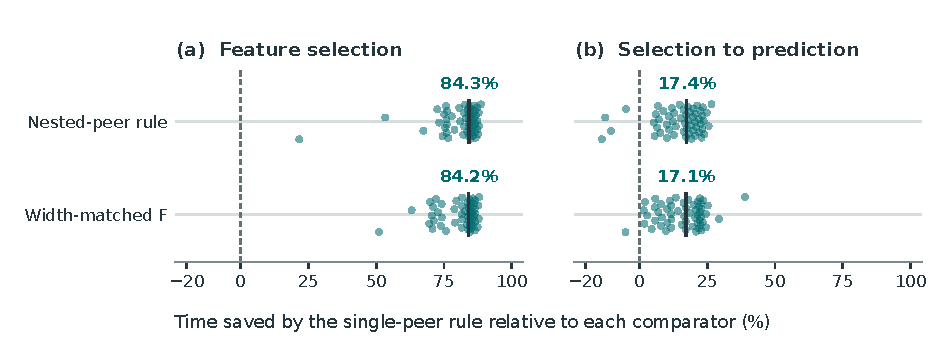
\includegraphics[width=\linewidth]{figures/lowdim-runtime.pdf}
\caption{Time saved by the single-peer rule against two supervised selectors on the 56 low-dimensional configurations. Each dot is one configuration. For each stage, its position gives the smaller percentage saving across the two timing processes. A point to the right of zero indicates a saving in both processes. Labeled vertical marks give the medians.}\label{fig:runtime}
\end{figure}

Table~\ref{tab:cases} gives the five-method comparison for two ten-column regression tasks. Abalone has seven numerical measurements and three indicator columns encoding sex~\cite{abalone}. In all 12 configurations, the single-peer rule kept all seven measurements and the same sex indicator. Collecting these eight columns still required all eight original attributes. All 12 configurations ran faster than Full. On the three original test splits, each evaluated with three selection seeds, the median paired time ratio was 0.940 and the mean loss in $R^2$ was 0.0000024. Diabetes had only 294 to 331 training rows per split. Five of its 11 configurations ran faster than Full in both processes, and mean $R^2$ fell by 0.01673. On all 23 Abalone and Diabetes configurations, the single-peer rule and the width-matched F filter selected exactly the same columns.

\begin{table}[htbp]\centering\small
\caption{Feature count $K$, mean test $R^2$, and median end-to-end time on the two ten-column regression tasks. Ranges give the smallest and largest $K$ across configurations.}\label{tab:cases}
\begin{tabular}{@{}lrrr@{\hspace{1.6em}}rrr@{}}
\toprule
 & \multicolumn{3}{c}{Abalone, 12 configurations} & \multicolumn{3}{c}{Diabetes, 11 configurations}\\
\cmidrule(lr){2-4}\cmidrule(l){5-7}
Method & $K$ & $R^2$ & Time (ms) & $K$ & $R^2$ & Time (ms)\\
\midrule
Single-peer rule & 8 & 0.52886 & 1.018 & 5--7 & 0.46770 & 1.044\\
Nested-peer rule & 3--7 & 0.47738 & 1.310 & 3--6 & 0.46543 & 1.263\\
Full & 10 & 0.52870 & 1.102 & 10 & 0.48443 & 1.082\\
Width-matched F & 8 & 0.52886 & 1.311 & 5--7 & 0.46770 & 1.308\\
Width-matched random & 8 & 0.51086 & 1.011 & 5--7 & 0.40045 & 1.049\\
\bottomrule
\end{tabular}
\tabnote{For each method and configuration, we averaged the two within-process median times. The table gives the median of these averages for each dataset. Equation~\eqref{eq:pair} compares the methods within each process before any aggregation across configurations.}
\end{table}

\subsection{Effect of the single-peer layer at fixed width}
In a separate ablation, we tested the peer layer on all 31 low-dimensional configurations in the original, supplementary, and eight-source repeated-holdout groups. We fixed the training-row sample and the width chosen by the single-peer rule. We then ranked columns using either the empty-peer gain in~\eqref{eq:empty} or the combined score in~\eqref{eq:score}. Including the peer layer changed seven selected sets. Test scores rose in two cases, tied in 28, and fell in one (Figure~\ref{fig:subsets}a). Both improvements occurred on Wisconsin Breast Cancer holdouts, with AUC gains of 0.00105 and 0.00084. The decrease occurred on a US macroeconomic split, where test $R^2$ for GDP fell by 0.04662.

\begin{figure}[!htbp]\centering
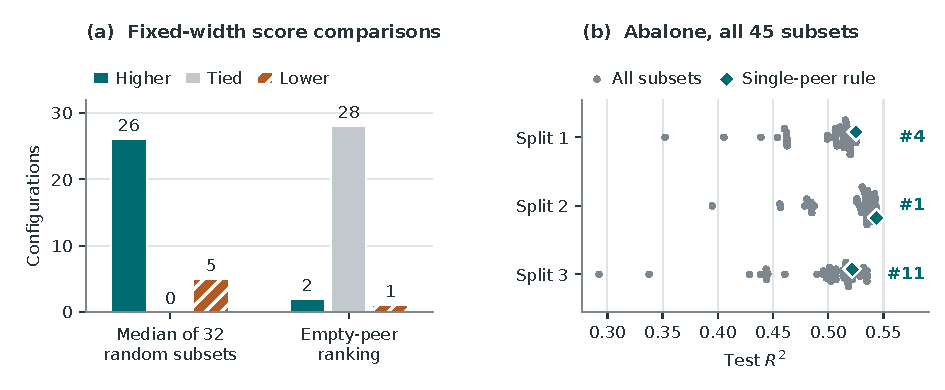
\includegraphics[width=\linewidth]{figures/subset-quality.pdf}
\caption{Test scores at matched width. (a) The 31 ablation configurations compare the single-peer rule with the median score of 32 uniform random subsets and with ranking by the empty-peer gain alone. (b) Each dot gives the test $R^2$ of one of the 45 eight-column subsets on an original Abalone split. Diamonds mark the subset selected by both the single-peer and empty-peer rules. All three seeds agreed within each split.}\label{fig:subsets}
\end{figure}

For each configuration we also drew 32 uniform random subsets at the same width. The single-peer rule scored above the median of those draws in 26 of 31 configurations. On Abalone we could enumerate all $\binom{10}{8}=45$ eight-column subsets. Ranking the refitted models by test $R^2$ placed the selected subset fourth, first, and eleventh on the three original test splits (Figure~\ref{fig:subsets}b). We used these rankings only for retrospective comparison. The empty-peer rule selected the same subset on each split, so the performance relative to random selection was already attainable from the marginal scores alone.

\FloatBarrier
\subsection{Score and runtime across all configurations}
The single-peer rule dropped at least one column in 384 of 387 configurations. It retained all 100 columns for each of the three selection seeds on the wheat-kernel protein task. In 231 configurations the reduced model ran faster than Full in both processes (Table~\ref{tab:tasks}). Of these, 106 matched or improved Full's test score. Allowing score losses of 0.01, 0.02, 0.05 and 0.10 increased the count to 140, 155, 180 and 195, respectively. Counting each combination of inputs, seed and primary metric once left 377 configurations, of which 225 reduced both width and runtime and 151 also met the 0.02 tolerance.

\begin{table}[htbp]\centering\small
\caption{Paired outcomes for the single-peer rule by prediction task. The two Full comparisons require both fewer columns and lower end-to-end time. The last two columns count a strictly higher test score and lower end-to-end time against the named baseline at the single-peer width. A time advantage must hold in both timing processes.}\label{tab:tasks}
\begin{tabular}{@{}lrrrrr@{}}
\toprule
 & & \multicolumn{2}{c}{Faster than Full} & \multicolumn{2}{c}{Higher score and faster}\\
\cmidrule(lr){3-4}\cmidrule(l){5-6}
Task & Cases & All & Loss $\le 0.02$ & vs.\ F & vs.\ random\\
\midrule
Binary classification & 178 & 105 & 71 & 41 & 0\\
Multiclass classification & 62 & 27 & 23 & 23 & 1\\
Regression & 147 & 99 & 61 & 41 & 4\\
\midrule
Total & 387 & 231 & 155 & 105 & 5\\
\bottomrule
\end{tabular}
\end{table}

The single-peer rule achieved a higher test score than the width-matched F filter in 155 configurations and a higher score than the fixed-seed random subset in 268. It was also faster than the respective baseline in 105 and five of these cases. No configuration gave a strict win in both score and time over both baselines. Using Full as the common reference, 106 single-peer, 102 F and 76 random subsets reduced both width and runtime and matched or improved Full's score. At the 0.02 tolerance the corresponding counts were 155, 128 and 159.

Figure~\ref{fig:matchedcurves} separates these outcomes by input width. In the low-dimensional group, the single-peer rule was faster than Full in 26 of 56 configurations, F in one and random selection in 30. Of these, 22, zero and 22, respectively, stayed within the 0.02 tolerance. Among the 331 wider configurations, the three methods were faster than Full in 205, 178 and 315 cases. Requiring a score loss of at most 0.02 left 133, 128 and 137 cases, respectively.

\begin{figure}[htbp]\centering
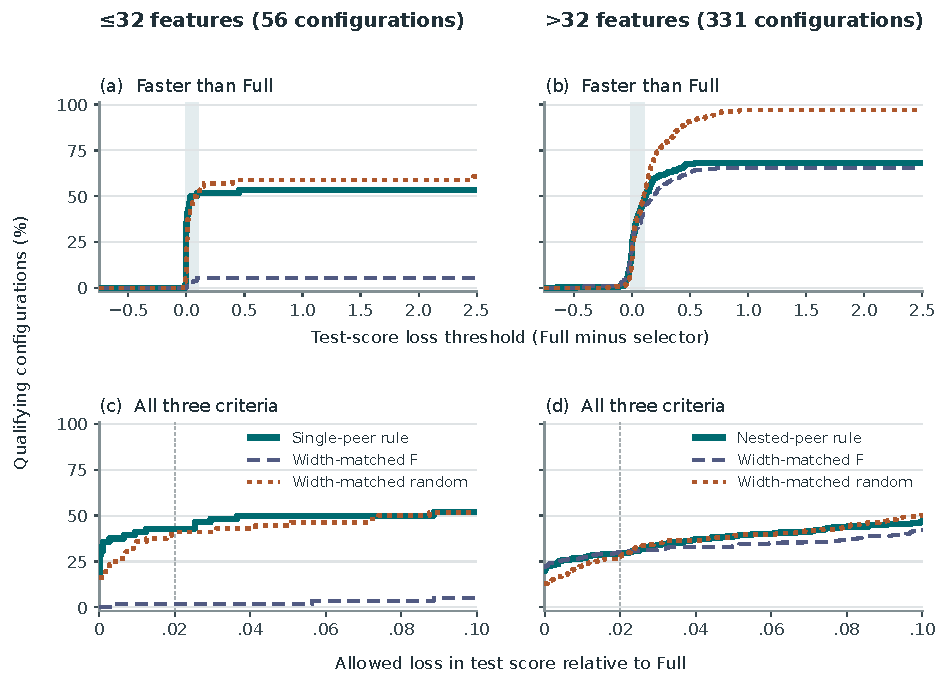
\includegraphics[width=\linewidth]{figures/matched-curves.pdf}
\caption{Single-peer selection and its width-matched baselines relative to Full. Each curve gives the share of all configurations in its width group that ran faster in both processes and lost at most the indicated test score (balanced accuracy, ROC AUC or $R^2$). Panels (a, b) cover all observed speedups. Negative loss indicates a score gain. Panels (c, d) also require fewer columns and enlarge the shaded interval from 0 to 0.10. The vertical guide marks a loss of 0.02.}\label{fig:matchedcurves}
\end{figure}

On the 331 wider inputs, single-peer selection produced a higher test score than the nested-peer comparator in 209 cases, the same score in four and a lower score in 118. The median fraction of columns retained was 46.1\% for single peers and 25.5\% for nested peers. The nested comparator reduced width and runtime in 222 cases, of which 93 stayed within the 0.02 tolerance. Single-peer selection reached that tolerance in 40 more cases while reducing width and runtime in 17 fewer. The two selectors chose their widths independently.

Across the 38 sparse text and advertising configurations, single-peer selection retained a median of 11.2\% of the columns. Balanced accuracy exceeded that of the width-matched random subset in 36 cases, with a mean advantage of 12.62 percentage points across all 38. It averaged 0.11 points below the F filter. Only four of the 38 single-peer pipelines finished sooner than Full in both processes. The median paired time ratios were 1.89 relative to Full, 2.56 relative to F and 5.55 relative to random selection. On near-infrared spectra, 15 of 36 configurations reduced both width and runtime, and nine of those 15 kept the $R^2$ loss within 0.02.

\FloatBarrier
\section{Discussion and conclusions}
Across the 331 wider configurations, the median end-to-end saving relative to Full was 10.7\% with single peers and 24.4\% with nested groups, taking the smaller saving in each pair of timing processes. Among the configurations that ran faster than Full, 36 of 205 single-peer subsets and 71 of 222 nested-peer subsets lost more than 0.10 on the primary test score. Three selection seeds on one mango spectroscopy split illustrate the trade-off. The median $R^2$ loss was 0.004 with single peers and 0.069 with nested groups, at median end-to-end times of 5.77 and 2.58~ms. Across the whole benchmark the two rules retained the same number of columns in 27 configurations. In 15 of these they chose different columns.

With rare outcomes, the metric also affects the comparison. The credit-card test set contained 98 fraudulent transactions among 56\,962 records. The single-peer rule kept eight of 29 columns and saved 59.6\% of the end-to-end time relative to Full in the less favorable timing process. ROC AUC fell from 0.97164 to 0.94218, and AP fell from 0.71707 to 0.69041. At the same default decision threshold, detections fell from 38 to 33. The width-matched F filter achieved an AUC of 0.91525 and an AP of 0.69186. On this single holdout, AUC favored the single-peer rule and AP favored F.

The timed runs used a warmed selector and predictor implementation in each of the two processes. On the 56 low-dimensional configurations, 14 saved at least 5\% of end-to-end time in each timing process and one saved at least 10\%. A separate cold-start measurement on this machine put the median cost of loading the small-matrix kernel at 0.850~ms across five fresh processes. The 387 configurations use ridge predictors on one machine with one numerical thread. Some sources contribute several seeds on the same test set, and some earlier Spambase holdouts contain identical feature vectors on both sides of the split. We chose the all-width single-peer policy after comparing the two rules on these same configurations. The policy comparison therefore describes this benchmark.

The single-peer rule and the F filter chose identical columns in all 23 Abalone and Diabetes configurations. Equation~\eqref{eq:bound} explains one circumstance in which an individual peer has little influence on the average. In the fixed-width ablation, adding the peer term improved two breast-cancer AUC scores and lowered one GDP $R^2$ score. At matched widths, random selection qualified in four more configurations than the single-peer rule when a loss of 0.02 was acceptable. With zero loss, the single-peer rule qualified in 30 more. The choice between them depends on the cost of a lower test score as well as the time available for selecting columns.

\begin{thebibliography}{9}\small\raggedright
\enlargethispage{\baselineskip}
\setlength{\itemsep}{0pt}
\bibitem{cohen} S. Cohen, G. Dror, and E. Ruppin. Feature selection via coalitional game theory. \emph{Neural Computation}, 19(7), 1939--1961, 2007. \href{https://doi.org/10.1162/neco.2007.19.7.1939}{doi:10.1162/neco.2007.19.7.1939}.
\bibitem{zhao} C. Zhao, J. Liu, and E. Parilina. Strategic inputs: feature selection from game-theoretic perspective. \emph{arXiv:2510.24982v2}, 2025. \url{https://arxiv.org/abs/2510.24982v2}.
\bibitem{kaur} J. N. Kaur, P. Patil, D. Shanmugam, E. Pierson, M. I. Jordan, N. Haghtalab, M. Jagadeesan, A. Alaa, and S. Wang. Strategic feature selection. \emph{arXiv:2606.18867v1}, 2026. \url{https://arxiv.org/abs/2606.18867v1}.
\bibitem{ridge} A. E. Hoerl and R. W. Kennard. Ridge regression: biased estimation for nonorthogonal problems. \emph{Technometrics}, 12(1), 55--67, 1970. \href{https://doi.org/10.1080/00401706.1970.10488634}{doi:10.1080/00401706.1970.10488634}.
\bibitem{pahikkala} T. Pahikkala, A. Airola, and T. Salakoski. Speeding up greedy forward selection for regularized least-squares. In \emph{Ninth International Conference on Machine Learning and Applications}, 325--330, 2010. \href{https://doi.org/10.1109/ICMLA.2010.55}{doi:10.1109/ICMLA.2010.55}.
\bibitem{rlscore} T. Pahikkala and A. Airola. RLScore: Regularized least-squares learners. \emph{Journal of Machine Learning Research}, 17(220), 1--5, 2016. \url{https://www.jmlr.org/papers/v17/16-470.html}.
\bibitem{skf} Scikit-learn developers. Univariate feature selection. \emph{Scikit-learn User Guide}, sec.~1.13.2. \href{https://scikit-learn.org/stable/modules/feature_selection.html}{scikit-learn.org, Feature selection}.
\bibitem{abalone} W. Nash, T. Sellers, S. Talbot, A. Cawthorn, and W. Ford. Abalone. \emph{UCI Machine Learning Repository}, 1995. \href{https://doi.org/10.24432/C55C7W}{doi:10.24432/C55C7W}.
\end{thebibliography}
\end{document}
